\documentclass[11pt]{article}

\usepackage{fullpage}
\usepackage{rotating}   
\usepackage{amsmath}
\usepackage{amssymb}
\usepackage{amsthm}
\usepackage{fancyhdr}
\usepackage{algorithm}
\usepackage{algorithmic}
\usepackage{bm}
\usepackage{listings}
\usepackage{graphicx}
\usepackage{caption2}
\usepackage{subfigure}
\usepackage{float}
\usepackage{extpfeil}
\usepackage{color}
\usepackage[usenames,dvipsnames]{xcolor}


\newtheorem{theorem}{Theorem}[section]
\newtheorem{lemma}[theorem]{Lemma}
\newtheorem{corollary}[theorem]{Corollary}
\newtheorem{proposition}[theorem]{Proposition}
\newtheorem{definition}[theorem]{Definition}
\newtheorem{conjecture}[theorem]{Conjecture}
\newtheorem{remark}[subsection]{Remark}

%%
\newcommand\numberthis{\addtocounter{equation}{1}\tag{\theequation}}

%% define new symbols
\def\bx{\bm{x}}
\def\bb{\bm{b}}
\def\ba{\bm{a}}
\def\bc{\bm{c}}
\def\bf{\bm{f}}
\def\by{\bm{y}}
\def\bu{\bm{u}}
\def\bv{\bm{v}}
\def\BW{\bm{W}}
\def\BA{\bm{A}}
\def\bz{\bm{z}}
\def\BZ{\bm{Z}}
\def\BH{\bm{H}}
\def\BL{\bm{L}}
\def\BU{\bm{U}}
\def\BV{\bm{V}}
\def\BB{\bm{B}}
\def\BC{\bm{C}}
\def\BD{\bm{D}}
\def\BE{\bm{E}}
\def\BW{\bm{W}}
\def\BQ{\bm{Q}}
\def\BG{\bm{G}}
\def\BA{\bm{A}}
\def\BX{\bm{X}}
\def\BY{\bm{Y}}
\def\BQ{\bm{Q}}
\def\BI{\bm{I}}
\def\BR{\bm{R}}

%% define new brackets
\def\la{\left\langle}
\def\ra{\right\rangle}
\def\ln{\left\|}
\def\rn{\right\|}
\def\lb{\left(}
\def\rb{\right)}
\def\lsb{\left[}
\def\rsb{\right]}
\def\lcb{\left\{}
\def\rcb{\right\}}

%%
\DeclareMathOperator*{\argmin}{arg\,min}
\DeclareMathOperator*{\argmax}{arg\,max}

%%
\title{Homework VI}
\author{Name: Shao Yanjun, Number: 19307110036}


\begin{document}
\maketitle

%------------------------------------
\begin{abstract}
This is Daniel's homework of  "Numerical Algorithms with Case Studies II".
\end{abstract}
%-------------------------------------
%=====================
\section{Problems}
\paragraph{Q1}
\subparagraph{(a)}
We have,
\begin{align}
	\frac{y}{a}&=e^{bx+cx^2}\\
	log(y)&-log(a)=bx+cx^2
\end{align}
If we reset $log(y)=\tilde{y}$, we will have a linear model,
\begin{align}
	\tilde{y}=\tilde{a}+bx+cx^2
\end{align}
\subparagraph{(b)}
We have,
\begin{align}
	\frac{1}{y}=1+e^{a+bx}\\
	log(\frac{1}{y}-1)=a+bx
\end{align}
If we reset $log(\frac{1}{y}-1)=\tilde{y}$, we will have a linear model,
\begin{align}
	\tilde{y}=a+bx
\end{align}
\subparagraph{(c)}
We have,
\begin{align}
	y=\frac{a}{(\frac{b}{\sqrt{x}}+1)^2}
\end{align}
If we reset $\frac{1}{\sqrt{y}}=\tilde{y}$ and $\frac{1}{\sqrt{x}}=\tilde{x}$ and $\sqrt{a}=\tilde{a}$, we will have a linear model,
\begin{align}
	\tilde{a}\tilde{y}=b\tilde{x}+1
\end{align}
\paragraph{Q2}
First check the semilogy() plot on bisection residuals, and we immediately discover that it should be fitted with $log(y)$ instead of $y$. Choose several basis \{$x,sin(x),cos(x),sin(2x),cos(2x),sin(3x),cos(3x)$\}
\begin{figure}[H]
	\centering
	\subfigure[residual]{
		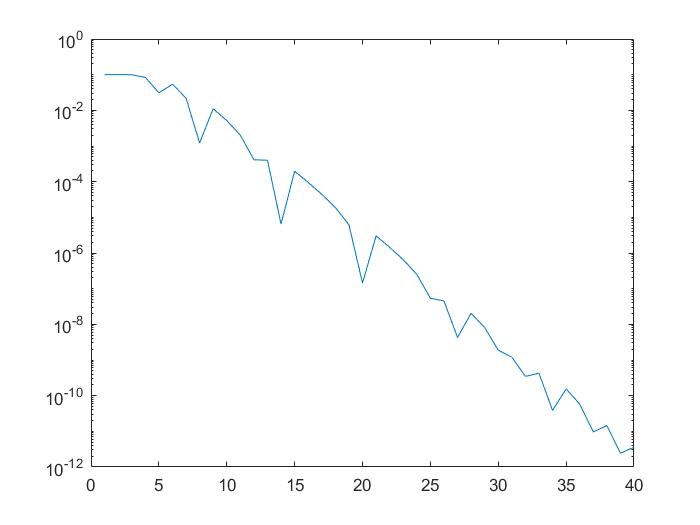
\includegraphics[width=0.4\linewidth]{bisection_loss.jpg}
	}
	\subfigure[fit]{
		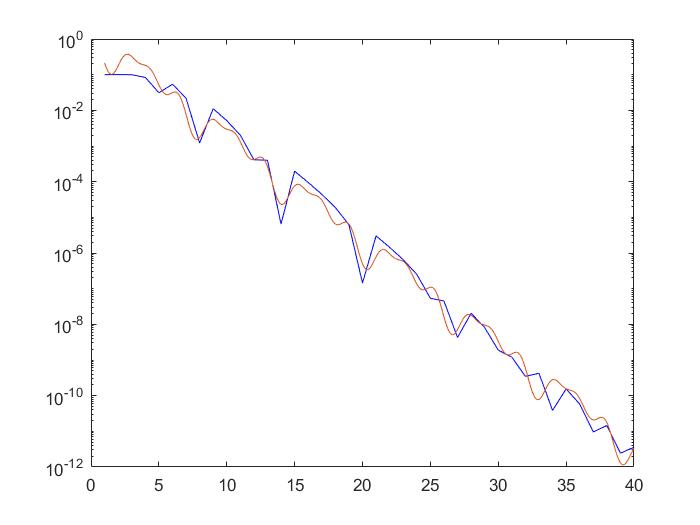
\includegraphics[width=0.4\linewidth]{bisection.jpg}
	}
\end{figure}
Next the residual of $regular$ $falsi$ is segmented into two parts.
\begin{figure}[H]
	\centering
	\subfigure[residual]{
		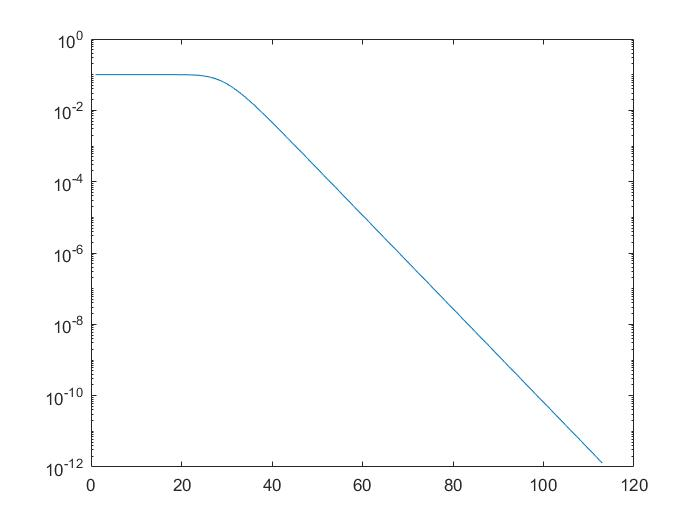
\includegraphics[width=0.4\linewidth]{regula_falsi_loss.jpg}
	}
	\subfigure[fit]{
		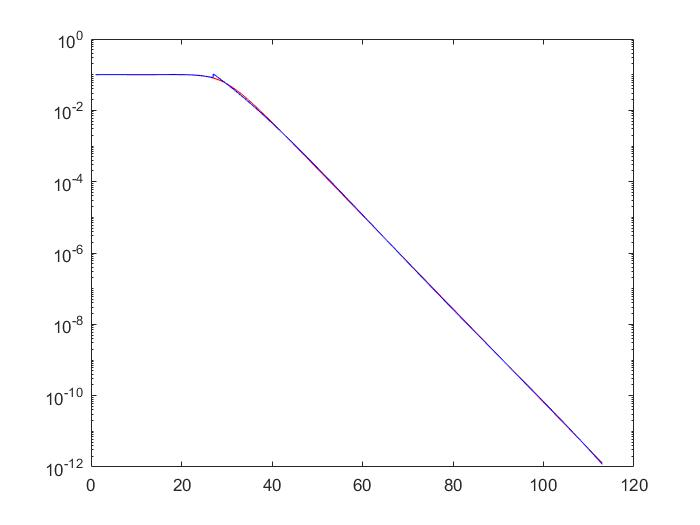
\includegraphics[width=0.4\linewidth]{regular_falsi.jpg}
	}
\end{figure}
\paragraph{Q3}
The most important thing of this model is that we must start our searching from two different basis with $\gamma_1=-\gamma_2$, because otherwise we are just trying to fit with only one basis, and can never converge to a good result (see the poor result).
\begin{figure}[H]
	\centering
	\subfigure[poor]{
		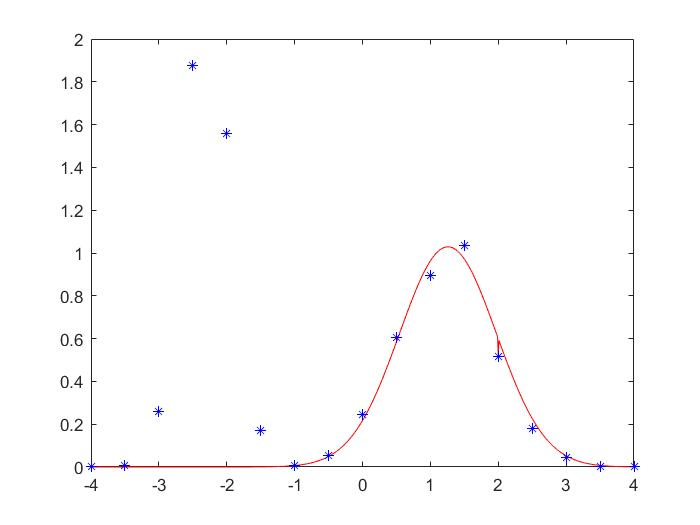
\includegraphics[width=0.4\linewidth]{poor.jpg}
	}
	\subfigure[good]{
	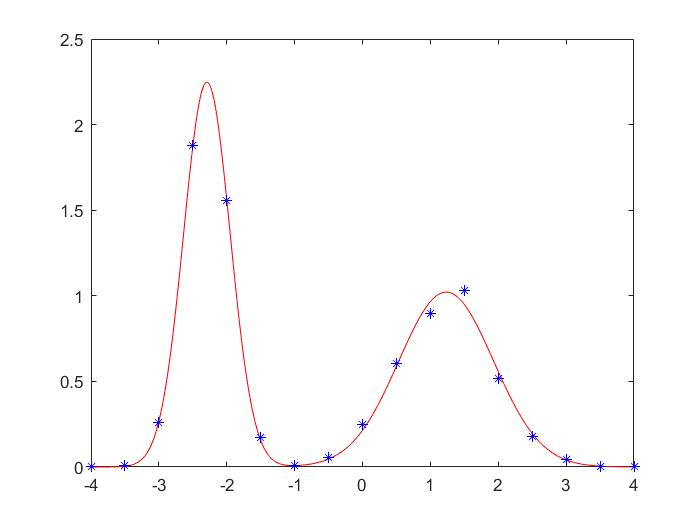
\includegraphics[width=0.4\linewidth]{good.jpg}
}
\end{figure}
Through experiment, I discover that $\alpha$ and $\beta$ are not so sensitive to initial values.
\paragraph{Q4}
We discover with joy that hyperbolic triangular functions have similar properties as basic triangular functions, i.e.
\begin{align}
	cosh(a+b)&=\frac{e^{a+b}+e^{-a-b}}{2}\\
	&=\frac{e^{a}+e^{-a}}{2}\cdot\frac{e^{b}+e^{-b}}{2}-\frac{e^{a}-e^{-a}}{2}\cdot\frac{e^{b}-e^{-b}}{2}\\
	&=cosh(a)\cdot cosh(b)-sinh(a)\cdot sinh(b)
\end{align}
We define Chebyshev polynomial on $(1,+\infty)$ as $T_n(x)=cosh(n\cdot arccosh(x))$. Check the assumption.
\begin{align}
	2xT_n(x)&=2cosh(arccosh(x))\cdot cosh(n\cdot arccosh(x))\\
	&=cosh((n+1)arccosh(x))+cosh((n-1)arccosh(x))\\
	&=T_{n-1}(x)+T_{n+1}(x)
\end{align}
%-------------------------------------
%=====================
\end{document}
